\documentclass[border=3pt]{standalone}
% Shared preamble for the standalone figures of qurl_explained.tex.
% Build a figure from this folder:   tectonic fig_<name>.tex
% Colours: blue = full precision (FP), orange = 8-bit.
\usepackage[T1]{fontenc}
\usepackage{lmodern}
\usepackage{amsmath,amssymb}
\usepackage[dvipsnames]{xcolor}
\usepackage{tikz}
\usetikzlibrary{positioning,arrows.meta,calc,decorations.pathreplacing}
\usepackage{pgfplots}
\pgfplotsset{compat=1.17}
\colorlet{fp}{RoyalBlue}
\colorlet{qb}{BurntOrange}
\colorlet{good}{ForestGreen}
\colorlet{bad}{BrickRed}
\newcommand{\pold}{\pi_{\mathrm{old}}}
\newcommand{\thold}{\theta_{\mathrm{old}}}
\newcommand{\qthold}{\hat\theta_{\mathrm{old}}}
\tikzset{
  box/.style={draw, rounded corners=3pt, align=center, inner sep=4pt, font=\small},
  arr/.style={-{Stealth[length=2.2mm]}, thick},
  lab/.style={font=\footnotesize, align=center},
}
\pgfplotsset{
  small axes/.style={
    tick label style={font=\footnotesize}, label style={font=\footnotesize},
    title style={font=\small}, every axis plot/.append style={line join=round}},
}

\begin{document}
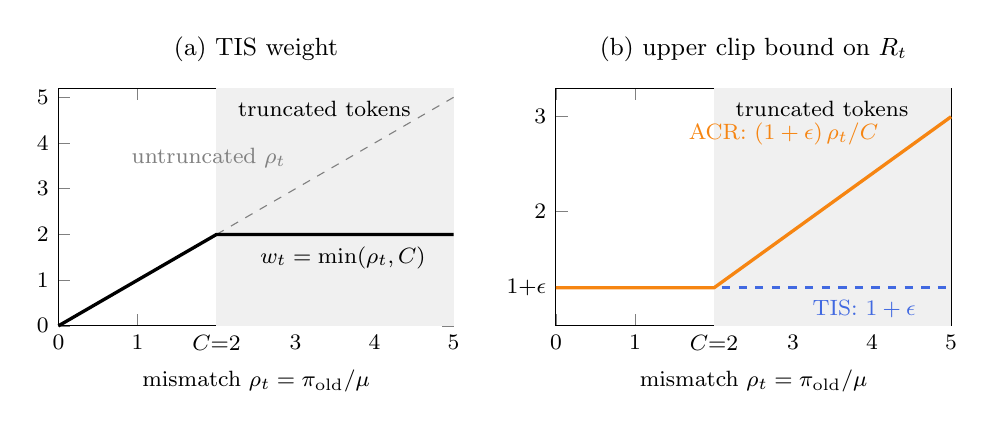
\begin{tikzpicture}
\pgfplotsset{tisax/.style={small axes, width=6.6cm, height=4.6cm, xmin=0, xmax=5, clip=false,
  xtick={0,1,2,3,4,5}, xticklabels={0,1,{$C{=}2$},3,4,5}, xlabel={mismatch $\rho_t=\pold/\mu$}}}
% (a) TIS weight
\begin{axis}[name=w, tisax, title={(a) TIS weight}, ymin=0, ymax=5.2, ytick={0,1,2,3,4,5}]
\fill[black!6] (axis cs:2,0) rectangle (axis cs:5,5.2);
\addplot[gray, dashed, domain=0:5] {x};
\addplot[black, very thick, domain=0:5, samples=101] {min(x,2)};
\node[lab, anchor=west] at (axis cs:2.15,4.75) {truncated tokens};
\node[lab, gray, anchor=south east] at (axis cs:3.0,3.25) {untruncated $\rho_t$};
\node[lab, anchor=north] at (axis cs:3.6,1.95) {$w_t=\min(\rho_t,C)$};
\end{axis}
% (b) upper clip bound on R_t
\begin{axis}[name=u, tisax, at={($(w.east)+(1.3cm,0)$)}, anchor=west, title={(b) upper clip bound on $R_t$},
  ymin=0.8, ymax=3.3, ytick={1.2,2,3}, yticklabels={$1{+}\epsilon$,2,3}]
\fill[black!6] (axis cs:2,0.8) rectangle (axis cs:5,3.3);
\addplot[fp, very thick, dashed, domain=0:5] {1.2};
\addplot[qb, very thick, domain=0:5, samples=101] {1.2*max(1,x/2)};
\node[lab, fp, anchor=north] at (axis cs:3.9,1.17) {TIS: $1+\epsilon$};
\node[lab, qb, anchor=south east] at (axis cs:4.2,2.6) {ACR: $(1+\epsilon)\,\rho_t/C$};
\node[lab, anchor=west] at (axis cs:2.15,3.08) {truncated tokens};
\end{axis}
\end{tikzpicture}
\end{document}
